% --------------------------------------------------------------
% This is all preamble stuff that you don't have to worry about.
% Head down to where it says "Start here"
% --------------------------------------------------------------
 
\documentclass[12pt]{article}
 
\usepackage[margin=1in]{geometry} 
\usepackage{amsmath,amsthm,amssymb}
\usepackage{enumerate}
\usepackage{graphicx}
\usepackage{pdfpages}
\usepackage{listings}
\graphicspath{{home/users/mark/Documents/school/ams 274/hw3}}
 
\newcommand{\N}{\mathbb{N}}
\newcommand{\Z}{\mathbb{Z}}
\newcommand{\R}{\mathbb{R}}

 
\newenvironment{theorem}[2][Theorem]{\begin{trivlist}
\item[\hskip \labelsep {\bfseries #1}\hskip \labelsep {\bfseries #2.}]}{\end{trivlist}}
\newenvironment{lemma}[2][Lemma]{\begin{trivlist}
\item[\hskip \labelsep {\bfseries #1}\hskip \labelsep {\bfseries #2.}]}{\end{trivlist}}
\newenvironment{exercise}[2][Exercise]{\begin{trivlist}
\item[\hskip \labelsep {\bfseries #1}\hskip \labelsep {\bfseries #2.}]}{\end{trivlist}}
\newenvironment{reflection}[2][Reflection]{\begin{trivlist}
\item[\hskip \labelsep {\bfseries #1}\hskip \labelsep {\bfseries #2.}]}{\end{trivlist}}
\newenvironment{proposition}[2][Proposition]{\begin{trivlist}
\item[\hskip \labelsep {\bfseries #1}\hskip \labelsep {\bfseries #2.}]}{\end{trivlist}}
\newenvironment{corollary}[2][Corollary]{\begin{trivlist}
\item[\hskip \labelsep {\bfseries #1}\hskip \labelsep {\bfseries #2.}]}{\end{trivlist}}
 
\begin{document}
 
% --------------------------------------------------------------
%                         Start here
% --------------------------------------------------------------
 
%\renewcommand{\qedsymbol}{\filledbox}
 
\title{AMS 274: HW4}%replace X with the appropriate number
\author{Mark Beers %replace with your name
} %if necessary, replace with your course title
 
\maketitle
 
\begin{enumerate}
\item Binary Response
\begin{enumerate}[(a)]
	\item Here we assume x is given, so we don't have to condition on x in the statement $P(Y = 1)$. We say that $P(Y=1)$ follows the logistic regression structure if $P(Y=1) = \Phi(x^T\beta)$.
	\begin{align*}
	P(Y=1) &= P(U_1 > U_0) \\
	&= P(a_1 + b_1 x +\epsilon_1 > a_0 + b_0 x + \epsilon_0) \\
	&= P((a_1 - a_0) + (b_1 - b_0)x > \epsilon_0 - \epsilon_1) \\
	&= P\bigg(\frac{1}{\sqrt{2}}[(a_1 - a_0) + (b_1 - b_0)x] > \frac{1}{\sqrt{2} }(\epsilon_0 - \epsilon_1)\bigg) \\
	\epsilon &= \frac{1}{\sqrt{2}} (\epsilon_0 - \epsilon_1) \sim N(0,1)  \\
	\implies P(Y=1) &=P\bigg(\epsilon < \frac{a_1 - a_0}{\sqrt{2}} + \frac{b_1 - b_0}{\sqrt{2}}x\bigg) = \Phi\bigg(\frac{a_1 - a_0}{\sqrt{2}} + \frac{b_1 - b_0}{\sqrt{2}}x\bigg)\\
	&= \Phi(\beta_0 +\beta_1x) \\
	\implies \beta_0 &= \frac{a_1 - a_0}{\sqrt{2}} \\
	\beta_1 &= \frac{b_1 - b_0}{\sqrt{2}}
	\end{align*}
	\item Now rather than following standard normal distributions, $\epsilon_1, \epsilon_0$ follow the gumbel distribution, with CDF $F(\epsilon_i) = exp(-exp(-\epsilon_i))$. The process of showing that this satisfies the logistic regression model structure proceeds much the same way as the normally distributed case. This time, we assume that $P(Y=1)$ satisfies the logistic regression model structure if $P(Y=1) = F(x^T\beta)$ where $F$ is the CDF of the logistic distribution. 
	\begin{align*}
	P(Y=1) &= P(U_1 > U_0)\\
	&= P((a_1 - a_0) + (b_1 - b_0)x > \epsilon_0 - \epsilon_1) 
	\end{align*}
	Now the question is what's the distribution of the difference of two Gumbel random variables. Below we show that the difference is a standard logistic distribution by characterizing the distribution using the moment generating function. 
	\begin{align*}
		E[e^{t(\epsilon_0 - \epsilon_1)}] &= E[e^{t\epsilon_0}e^{-t\epsilon_1}] \\
		&= E[e^{t\epsilon_0}]E[e^{-t\epsilon_1}] \quad\text{$\epsilon_0, \epsilon_1$ independent.}\\
		E[e^{t\epsilon_0}] &= \int_{-\infty}^{\infty} e^{t\epsilon_0} exp(-exp(-\epsilon_0)) e^{-\epsilon_0} d\epsilon_0 \\ 
		&= \int_{0}^{\infty} u^{(1-t) -1}e^{-u} du = \Gamma(1-t), \quad \text{$u = e^{-x}$}\\
		E[e^{-t\epsilon_1}] &= \int_{-\infty}^{\infty} e^{-t\epsilon_1} exp(-exp(-\epsilon_1)) e^{-\epsilon_1} d\epsilon_0 \\ 
		&= \int_{0}^{\infty} u^{(1+t) -1}e^{-u} du = \Gamma(1+t),  \quad \text{$u = e^{-x}$}\\
		E[e^{t\epsilon_0}]E[e^{-t\epsilon_1}] &=\Gamma(1+t)\Gamma(1-t) = \frac{\Gamma(1+t)\Gamma(1-t)}{\Gamma((1+t) + (1-t))} = B(1+t, 1-t) 	
\end{align*}
So the moment generating function of the difference of two gumbel distributed random variables is $B(1+t, 1-t)$ where B is the beta function. Now we will show that the MGF of a standard logistic random variable is exactly this using an integral result from the beta function page on wikipedia. 
\begin{align*}
M_X(t) &= \int_{-\infty}^{\infty} \frac{e^{-x}}{(1 + e^{-x})^2}e^{tx} dx \\
&= \int_{0}^{\infty}\frac{u^{(1-t)-1}}{(1+u)^{(1-t)+(1+t)}} du \quad \text{$u = e^{-x}$} \\
&= B(1-t, 1+t) \quad \text{Wikipedia integral result}
\end{align*}
So the MGF of the difference of two standard gumbel distributed random variables is equal to the MGF of a standard logistic distribution. By the uniqueness of the MGF, $\epsilon_0 - \epsilon_1 \sim logistic(0,1)$. So, 
\begin{align*}
P(Y=1) &= P(U_1 > U_0)\\
&= P((a_1 - a_0) + (b_1 - b_0)x > \epsilon_0 - \epsilon_1)  \\
&= P(\epsilon< (a_1 - a_0) + (b_1 - b_0)x), \quad \epsilon \sim logistic(0,1) \\
&=F((a_1 - a_0) + (b_1 - b_0)x), \quad \text{F is a logistic CDF} \\
&= F(\beta_0 + \beta_1 x) \\
\implies \beta_0 &= a_1 - a_0 \\
\beta_1 &= b_1 - b_0
\end{align*}

\end{enumerate}

\item Alligator Food Choice. Before we start part a, I include a histogram of length by food preference. Normally I would use empirical proportions to empirically validate our predicted probabilities, but $m_i$ is one here, so empirical proportions don't really apply. We note that the largest alligators strongly prefer fish, and that small alligators like to eat invertebrates. We hope to see this replicated in our predicted response probabilities, with long alligators having a high probability of preferring fish, and short alligators having a high probability of preferring invertebrates.\\
\newline
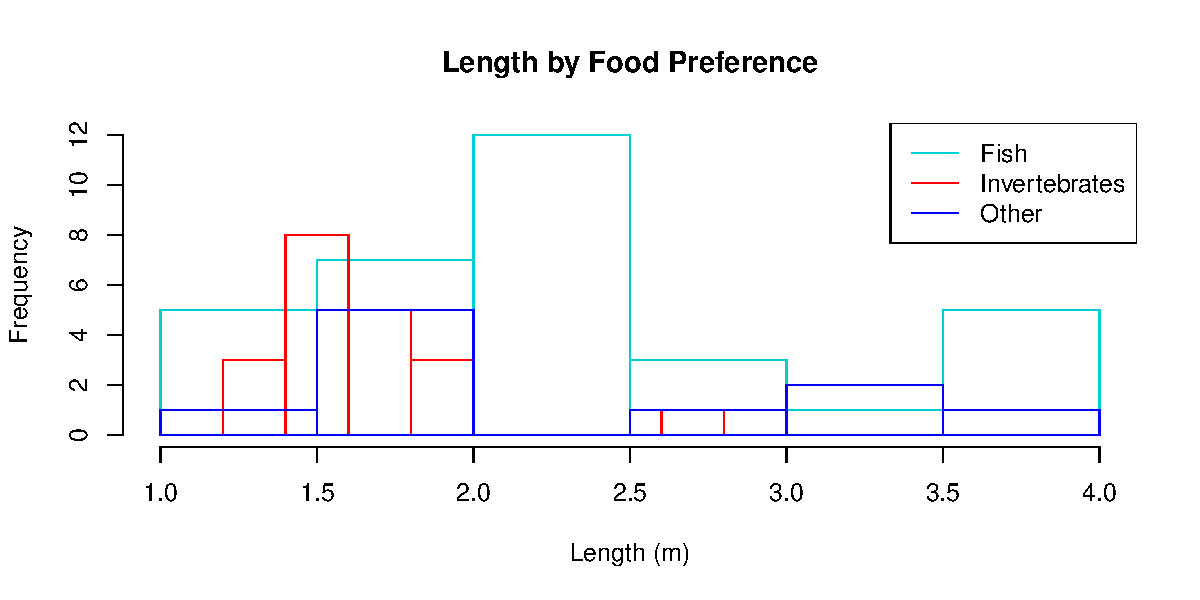
\includegraphics[scale = .7]{plot1.pdf} 



\begin{enumerate}[(a)]
	\item Here we focus on length as a single covariate to explain an alligator's preference for fish, invertebrates or other. We develop a Bayesian multinomial regression model, using the Metropolis Hastings algorithm to obtain posterior samples of the desired coefficients. Fish was used as the baseline category. In an effort to have uninformative priors, we use very dispersed, nearly flat independent normal priors for each covariate, with mean 0 and standard deviation 100. Candidate parameter values were generated from a multivariate normal. The corresponding variance covariance matrix was given by the negative inverse of the hessian matrix that the optim function applied to the log likelihood in R provides. Plots of the posterior samples are provided below. Posterior estimates are based on 10000 posterior samples, with the first 5000 thrown away. Blue lines indicate the mean of the posterior samples, green lines indicate the MLE, red lines indicate 95 percent confidence regions.  \\
	\newline
	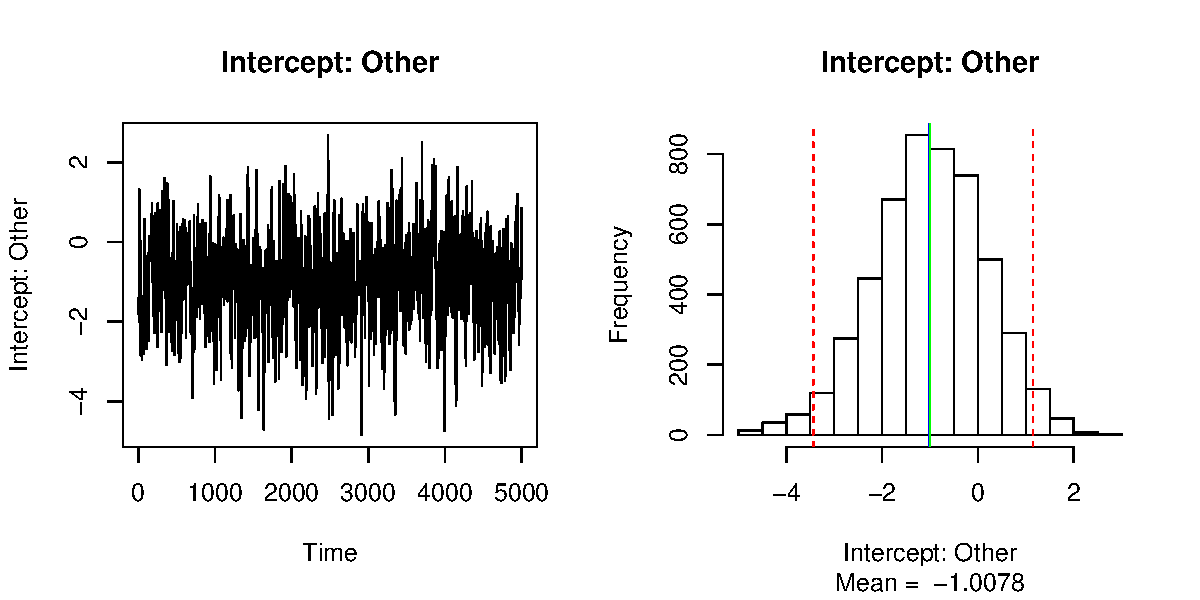
\includegraphics[scale = .7]{plot3.pdf} \\
	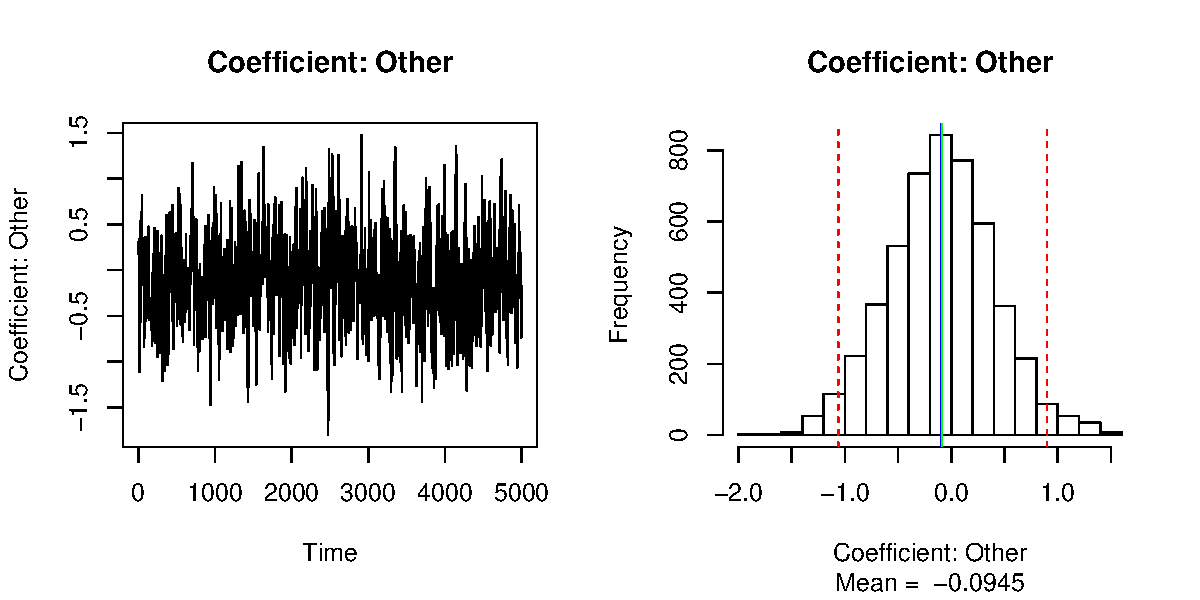
\includegraphics[scale = .7]{plot4.pdf} \\
	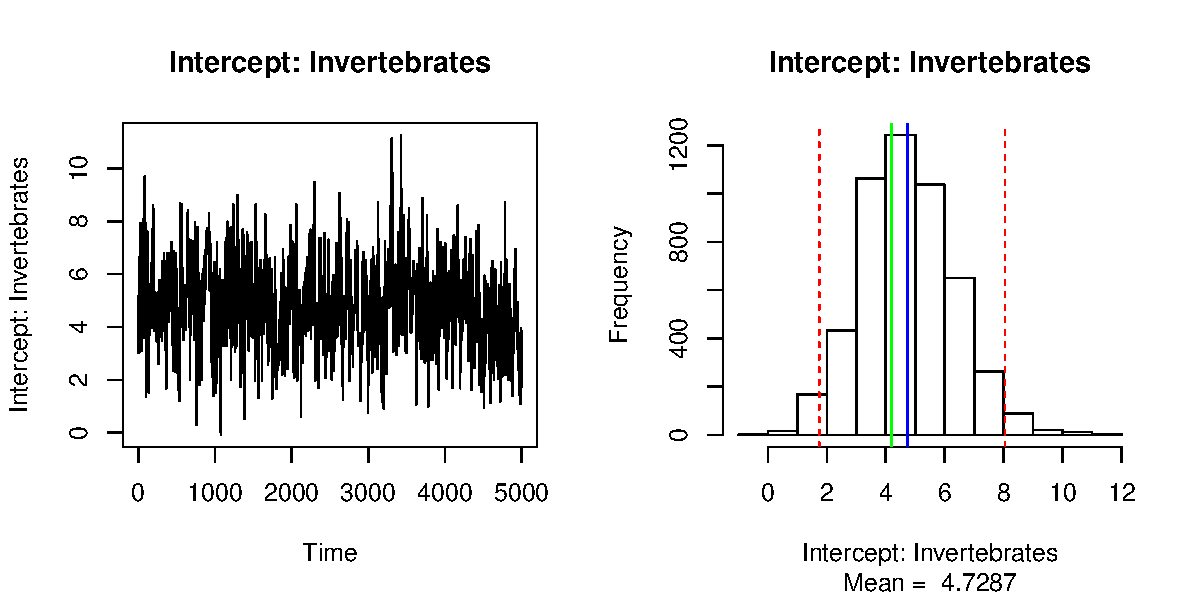
\includegraphics[scale = .7]{plot5.pdf} \\
	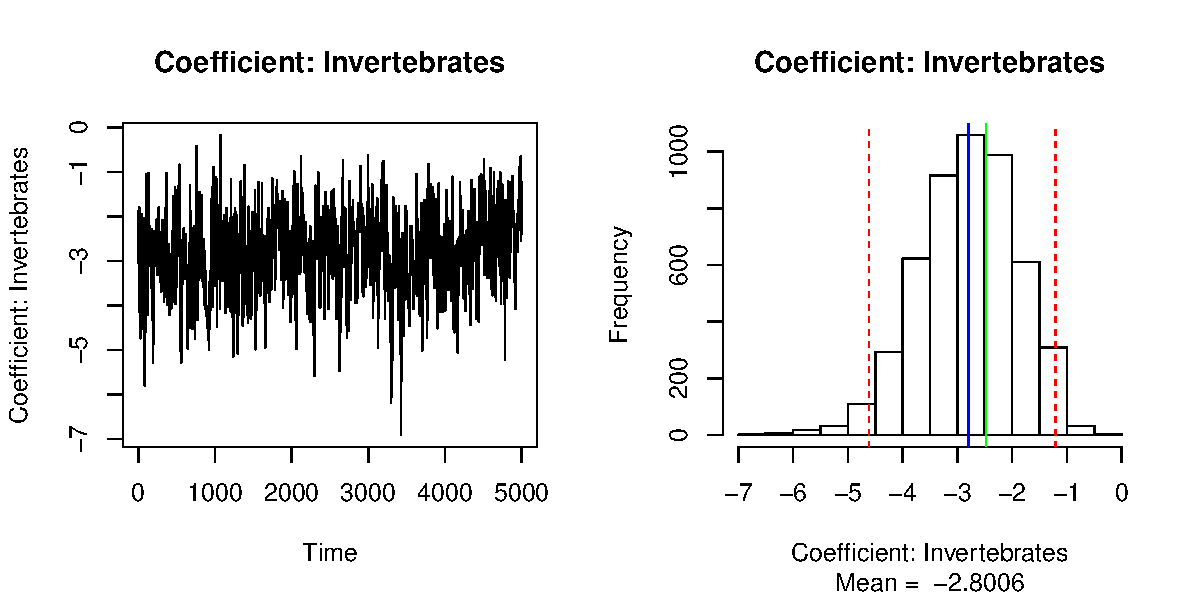
\includegraphics[scale = .7]{plot6.pdf} \\
	Using these posterior samples, we estimate response probabilities as a function of length. These probabilities are calculated using the following equations for some given length x. 
	\begin{align*}
	\pi_I &= \frac{exp(\alpha_I + \beta_I x)}{1 + exp(\alpha_I + \beta_I x) + exp(\alpha_O + \beta_O x)} \\ 
	\pi_O &= \frac{exp(\alpha_O + \beta_O x)}{1 + exp(\alpha_I + \beta_I x) + exp(\alpha_O + \beta_O x)} \\
	\pi_F &= \frac{1}{1 + exp(\alpha_I + \beta_I x) + exp(\alpha_O + \beta_O x)}  
	\end{align*}
	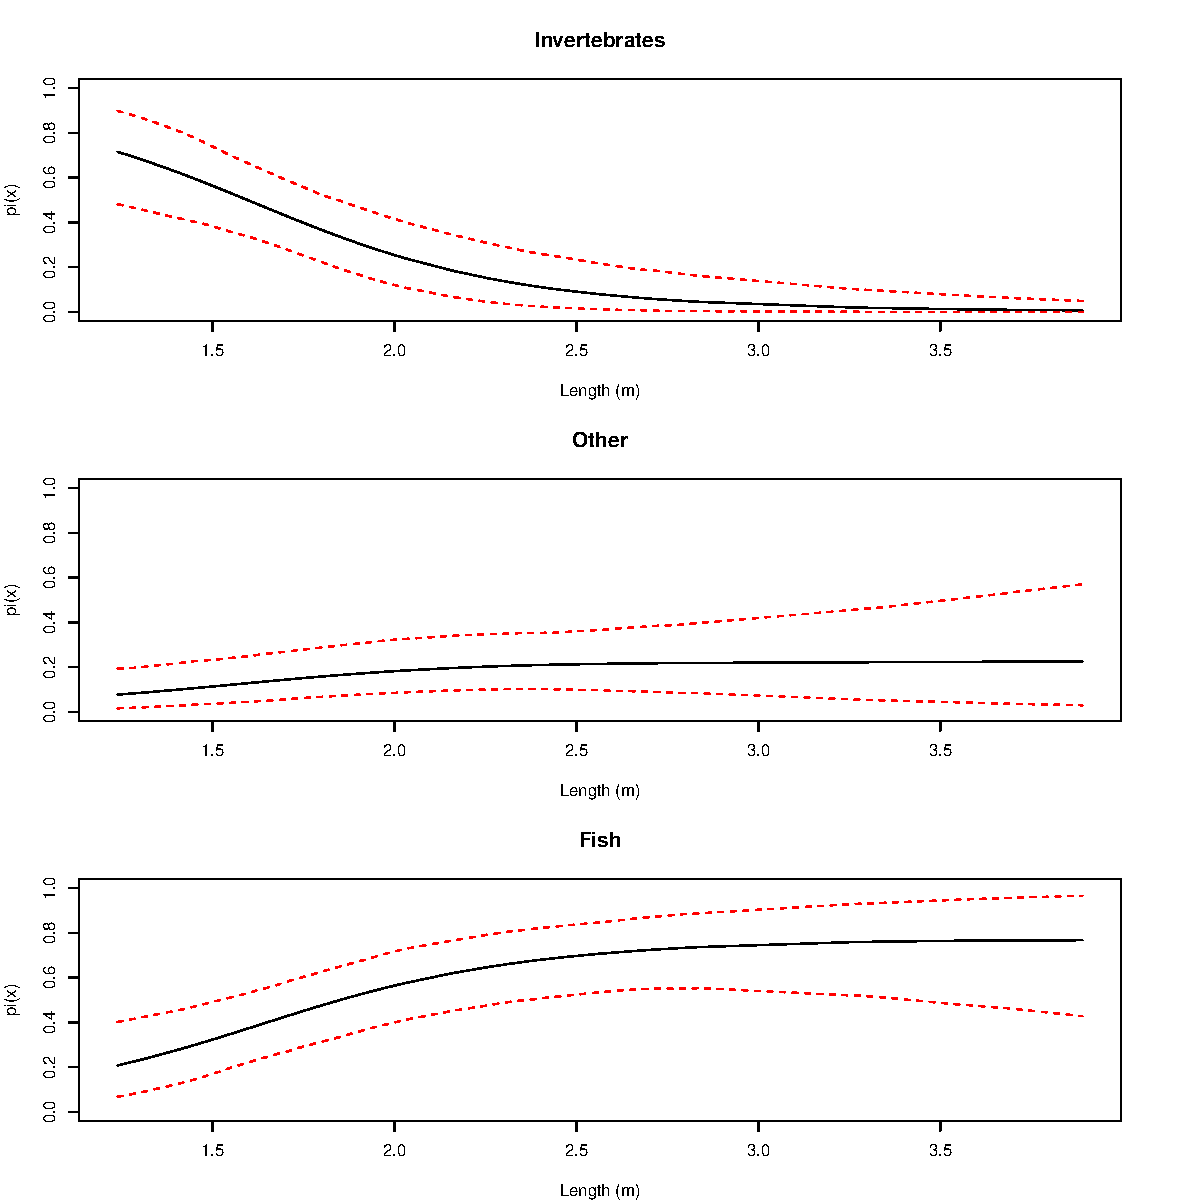
\includegraphics[scale = .7]{plot2.pdf} \\
	We note as expected that Fish are strongly preferred by large alligators and Invertebrates are preferred by small alligators. 
	
	
	\item Here we extend the model from part (a) to describe the effects of both length and gender on food choice. Similar plots of posterior samples are again provided below. MLEs were calculated, as before using the optim function in R with BFGS as the method. This approach was more robust to different initial starting points than the default Nelder Mead method which was interesting. \\
	\newline
	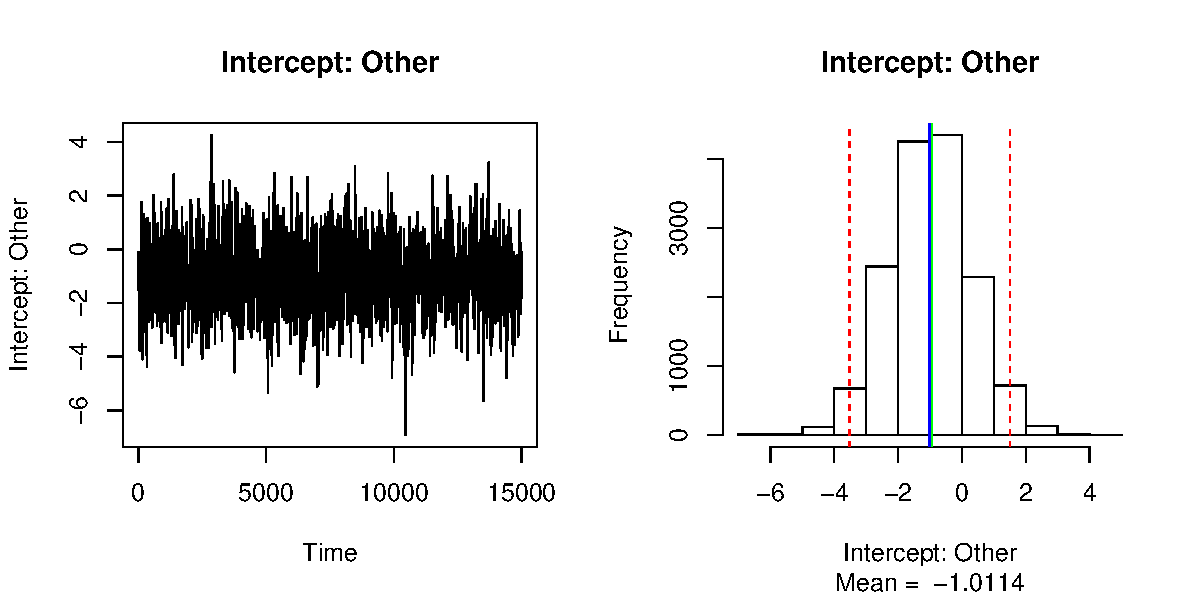
\includegraphics[scale = .7]{plot7.pdf} \\
	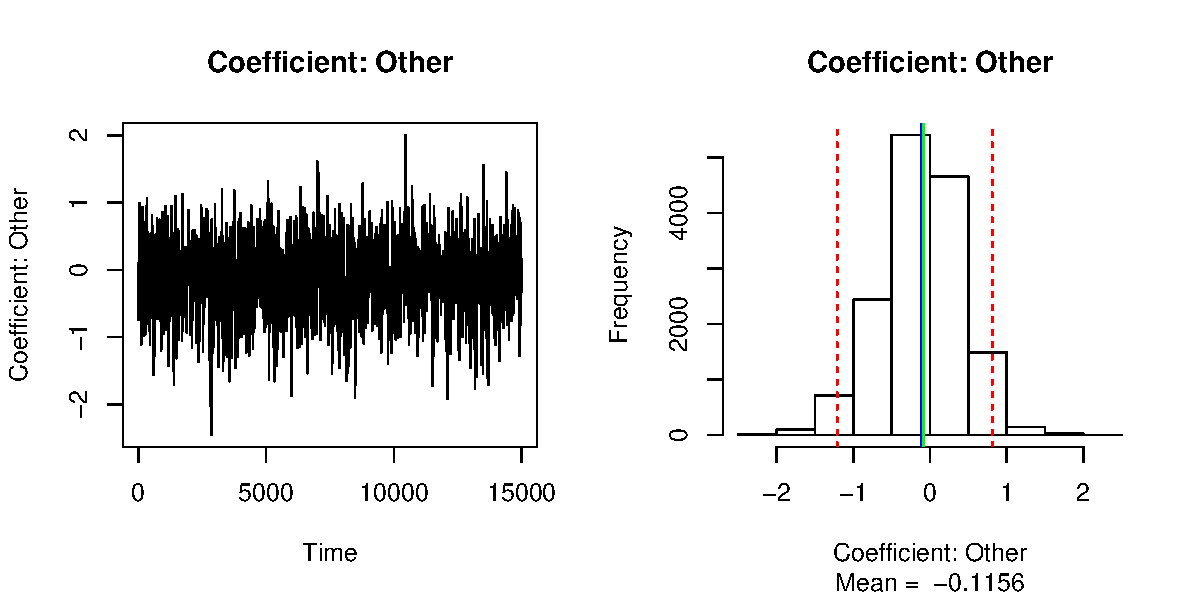
\includegraphics[scale = .7]{plot8.pdf} \\
	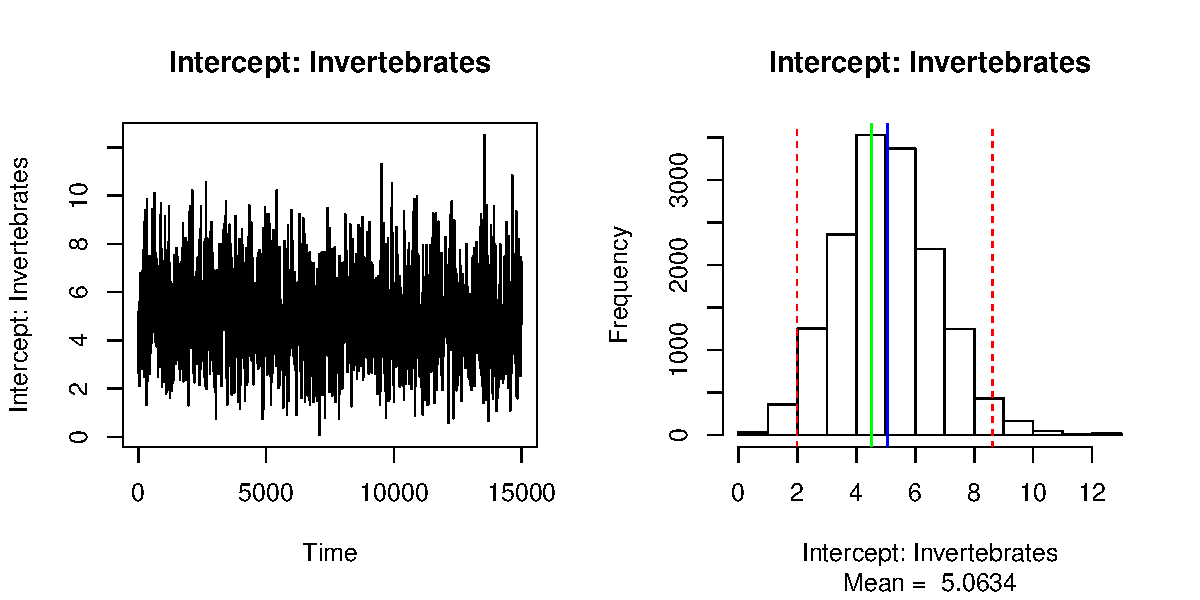
\includegraphics[scale = .7]{plot9.pdf} \\
	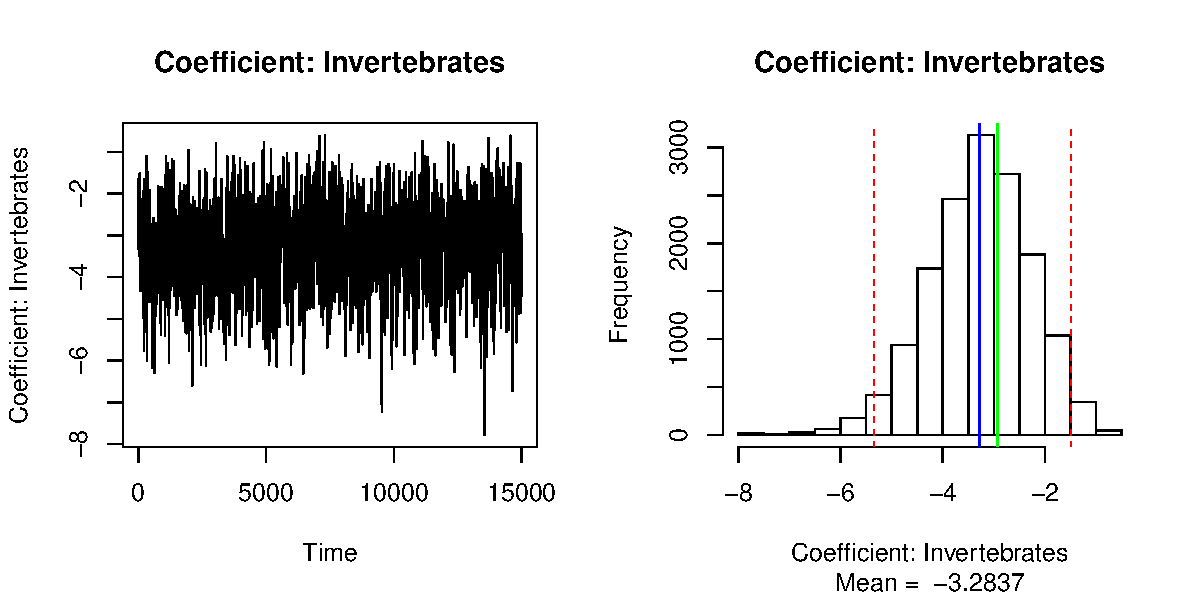
\includegraphics[scale = .7]{plot10.pdf} \\
	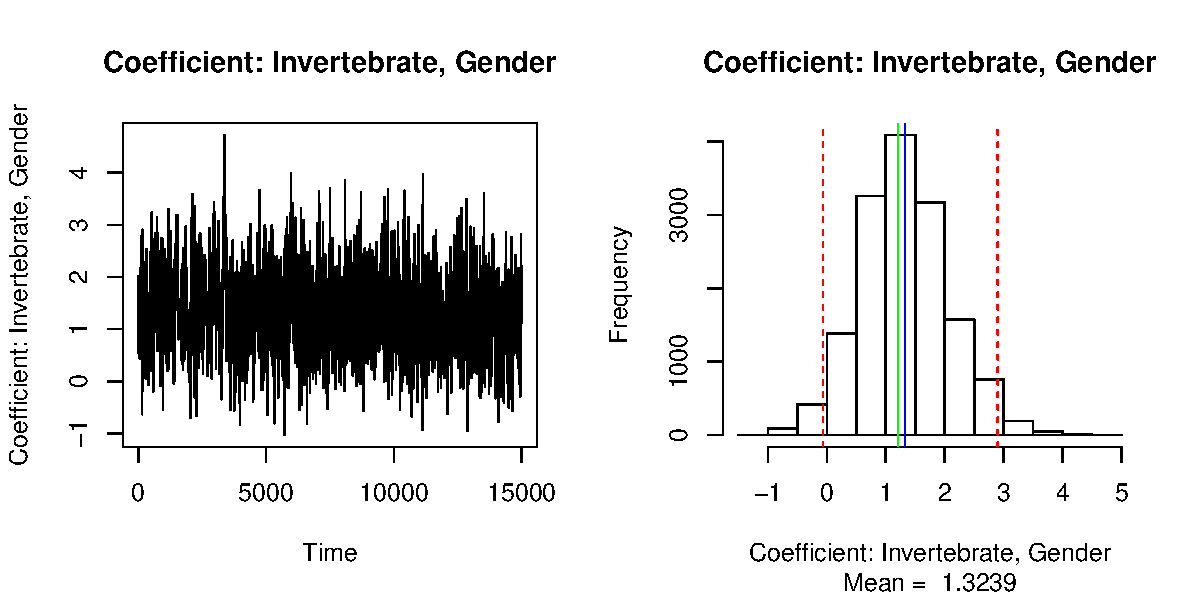
\includegraphics[scale = .7]{plot11.pdf} \\
	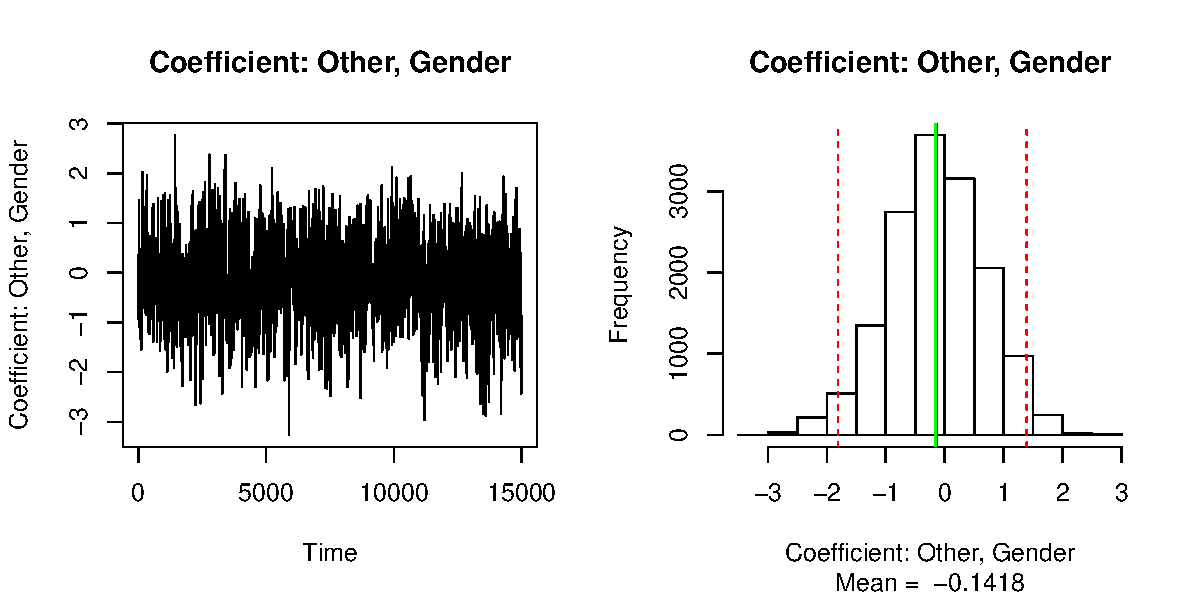
\includegraphics[scale = .7]{plot211.pdf} \\
	Using these posterior probabilities, we again compute length dependent  response probabilities, by gender. \\
	\newline
	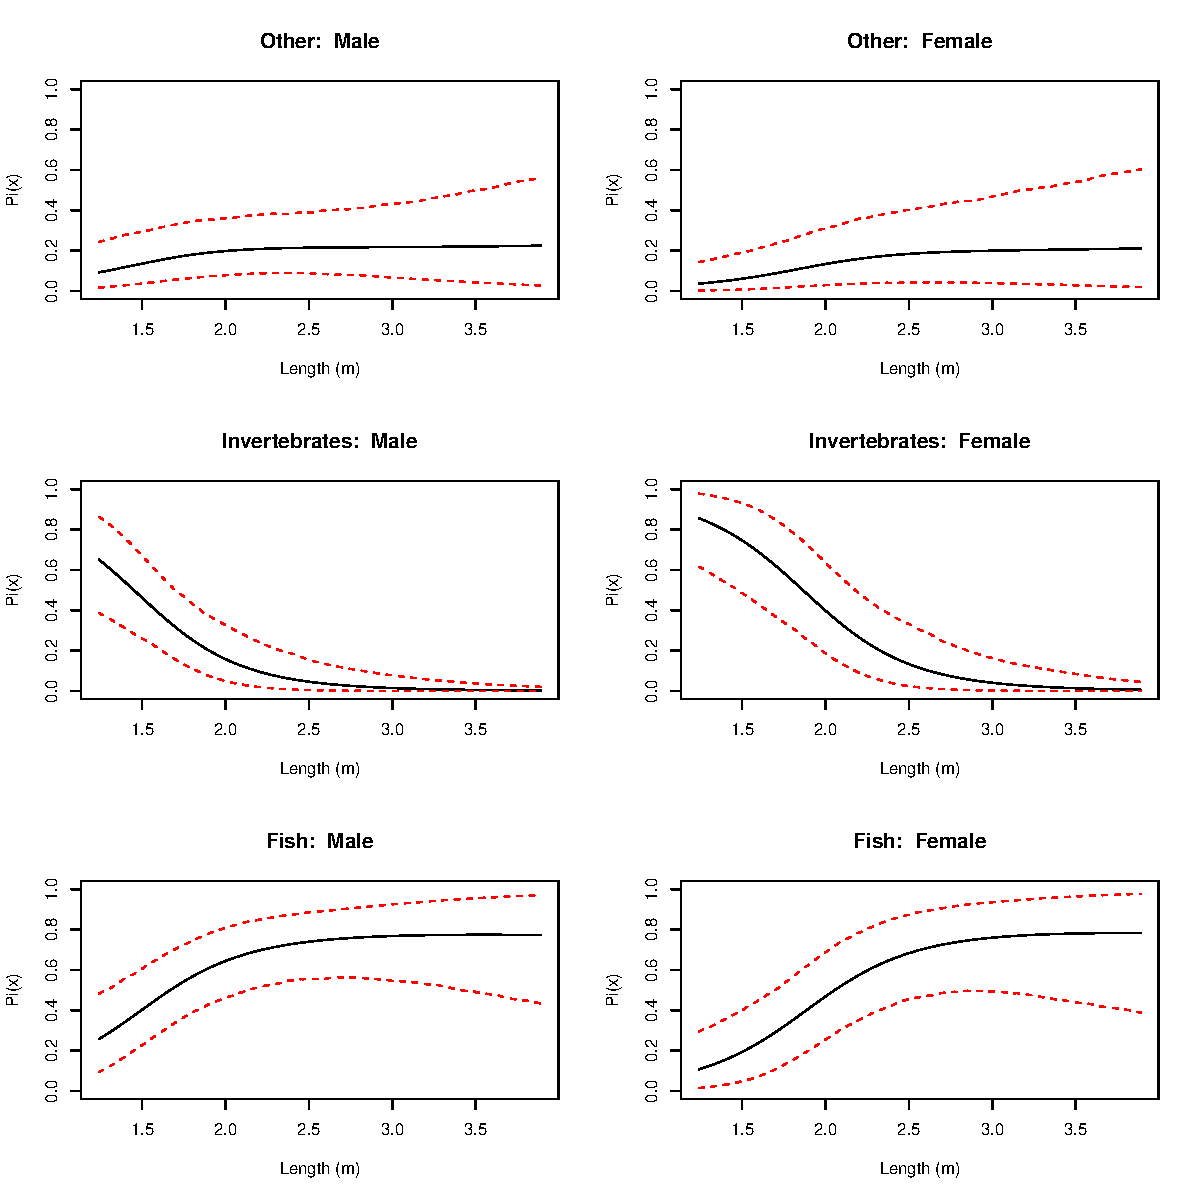
\includegraphics[scale = .7]{plot12.pdf} \\
	Again we note as expected that small alligators prefer invertebrates and large alligators prefer fish. We note that in particular, small female alligators prefer invertebrates, but large alligators, regardless of gender seem to prefer fish. 
	
	
\end{enumerate}


\item Developmental Toxicity. \\
\begin{enumerate}
	\item Below we go through an argument for why, in the case of continuation ratio logits, we can decompose our multinomial glm into two distinct Binomial GLMs. 
	\begin{align*}
	&Multinomial(y_1, y_2, y_3|m, \pi_1, \pi_2, \pi_3) \\&= \frac{m!}{y_1!y_2!(m-y_1 - y_2)!}\pi_1^{y_1}\pi_2^{y_2} (1- \pi_1 - \pi_2)^{m-y_1-y_2} \\
	&=\frac{m!}{y_1!(m-y_1)!} \frac{(m-y_1)!}{y_2!(m-y_1-y_2)!}\pi_1^{y_1}(1-\pi_1)^{m-y_1} \frac{1}{(1-\pi_1)^{m-y_1}} \pi_2^{y_2}(1-\pi_1-\pi_2)^{m-y_1-y_2} \\
	&= \binom{m}{y_1} \pi_1^{y_1}(1-\pi_1)^{m-y_1} \binom{m-y_1}{y_2}\bigg(\frac{1-\pi_1-\pi_2}{1-\pi_1}\bigg)^{m-y_1-y_2} \bigg(\frac{\pi_2}{1-\pi_1}\bigg)^{y_2} \\
	&= \binom{m}{y_1} \pi_1^{y_1}(1-\pi_1)^{m-y_1} \binom{m-y_1}{y_2}\bigg(\frac{\pi_3}{\pi_2 + \pi_3}\bigg)^{m-y_1-y_2} \bigg(\frac{\pi_2}{\pi_2 + \pi_3}\bigg)^{y_2} \\
	&= Bin(y_1|m, \frac{\pi_1}{\pi_1 + \pi_2 +\pi_3})\ Bin(y_2|m-y_1, \frac{\pi_2}{\pi_2 + \pi_3}) \\
	&= Bin(y_1|m, p_1)\ Bin(y_2|m-y_1, p_2) \\
	&p(y_1|m, \pi_1)p(y_2|m, \pi_1, \pi_2) = exp\bigg[y_1log\bigg(\frac{\pi_1}{1-\pi_1}\bigg) + mlog(1-\pi_1) + log\binom{m}{y_1}+ \\
	&\qquad\qquad y_2 log(\frac{\pi_2}{\pi_2 + \pi_3}) + (m- y_1 - y_2)log(\frac{\pi_3}{\pi_2 + \pi_3}) + log\binom{m-y_1}{y_2}\bigg] \\ 
	&= exp\bigg[y_1log\bigg(\frac{\pi_1}{\pi_2 + \pi_3}\bigg) + mlog(1-\pi_1) + log\binom{m}{y_1}+ \\ 
	&\qquad\qquad y_2 log(\frac{\pi_2}{\pi_3}) + (m-y_1)log(\frac{\pi_3}{\pi_2 + \pi_3}) + log\binom{m-y_1}{y_2} \bigg]
	\end{align*}
	So, basically we established that the multinomial likelihood can be decomposed into two binomial likelihoods. One of those likelihoods depends only on $\pi_1$ and the other depends only on $\pi_2$ and $\pi_3$ so, because there's no overlap of the $\pi_i$ in the glms, we can fit the two binomial glms separately. 
	So, including indexes now, we define the glm with the following components. 
	\begin{align*}
	\theta_{1i} &= g(\mu_{1i}) = log\bigg(\frac{\pi_1(x_i)}{\pi_2(x_i) + \pi_3(x_i)}\bigg) = \alpha_1 + \beta_1 x_i\\
	\theta_{2i} &= g(\mu_{2i}) = log\bigg(\frac{\pi_2(x_i)}{\pi_3(x_i)}\bigg) = \alpha_2 + \beta_2 x_i\\
	Y_i &= (y_{i1}, y_{i2},y_{i3}) \\
	\hat{\pi}_1(x_i) &= \frac{exp(\alpha_1 + \beta_1 x_i)}{1 + exp(\alpha_1 + \beta_1 x_i)} \\ 
	\hat{\pi}_2(x_i) &= \frac{exp(\alpha_2 + \beta_2 x_i)}{(1 + exp(\alpha_1 + \beta_1 x_i)(1 + exp(\alpha_2 + \beta_2 x_i))} \\
	\hat{\pi}_3(x_i) &= \frac{1}{(1 + exp(\alpha_1 + \beta_1 x_i)(1 + exp(\alpha_2 + \beta_2 x_i))}
	\end{align*}
	So, because we can decompose the multinomial likelihood into a product of two binomial likelihoods, one of which depends only on $\pi_1$, and the other that depends only on $\pi_2, \pi_3$, that just so happen to take the form used for continuous ratio logits, we can fully fit this model using two separate Binomial GLMs, which take the forms given above.
	\item Now that we've established this particular model can be fit using two separate binomial GLMs, we will obtain MLE estimates and corresponding standard errors for $\alpha_1, \alpha_2, \beta_1, \beta_2$. MLE estimates and standard errors are obtained using the optim function in R applied to the following log likelihoods. 
	\begin{align*}
	LL_1 &= log\bigg[\prod_{i=1}^{5} Bin(y_{1i}|m_i, \pi_1)\bigg] = \sum_{i=1}^{5} log\bigg[Bin(y_{1i}|m_i, \pi_1)\bigg] \\ 
	LL_2 &= log\bigg[\prod_{i=1}^{5} Bin(y_{2i}|m_i-y_{1i}, \frac{\pi_2}{\pi_2 + \pi_3})\bigg] = \sum_{i=1}^{5} log\bigg[Bin(y_{2i}|m_i-y_{1i}, \frac{\pi_2}{\pi_2 + \pi_3})\bigg]
	\end{align*}
	To get standard errors, we use the asymptotic result that $\hat{\beta}$ is asymptotically distributed as $N_p(\beta, J^{-1}(\hat{\beta}))$, where J is the observed fisher information matrix evaluated at the MLEs. From the optim function in R, we can get the appropriate hessian, which we multiply by -1, invert, and then take the square root of the diagonal elements of to get standard errors for the $\alpha_i, \beta_i$. Those results are provided in the table below. 
	\begin{table}[htb]
		\centering
		\begin{tabular}{|l|l|l|}
			\hline
			Coefficient & MLE          & SE           \\ \hline
			$\alpha_1$  & -3.248202248 & 0.1588523248 \\ \hline
			$\beta_1$   & 0.006389104  & 0.0004454399 \\ \hline
			$\alpha_2$  & -5.70135555  & 0.324514723  \\ \hline
			$\beta_2$   & 0.01737291   & 0.001185534  \\ \hline
		\end{tabular}
	\end{table}
	
	We will also plot the estimated response curves $\hat{\pi}_j(x)$ for $j = 1, 2,3$. \\
	\newline
	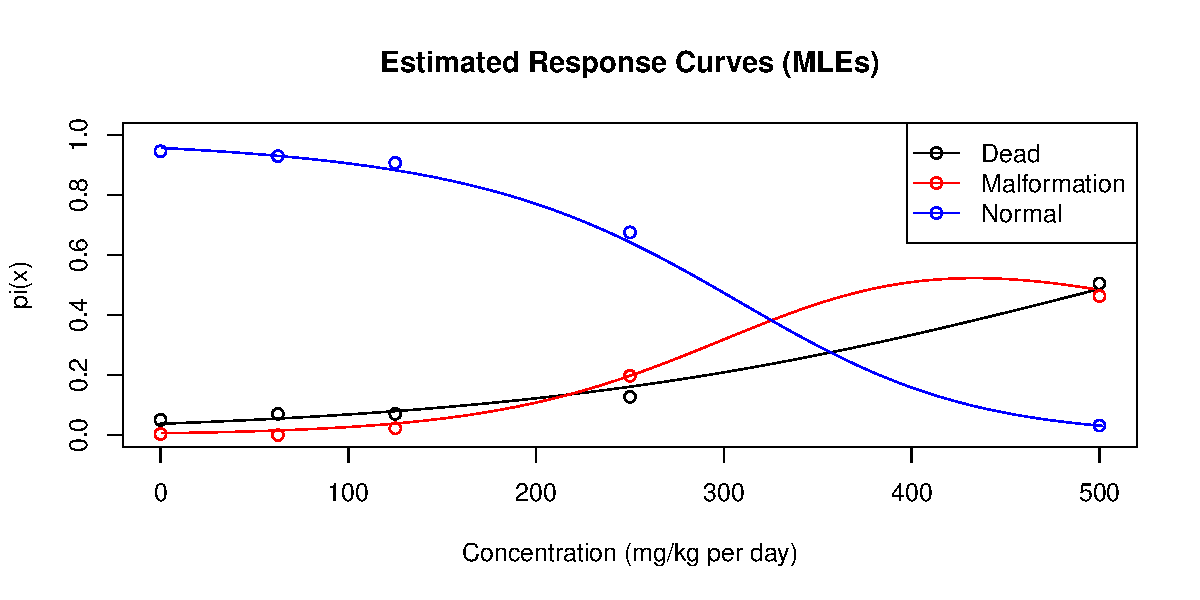
\includegraphics[scale = .7]{plot13.pdf} \\
	The dots  on the plot abovecorrespond to the observed proportions. We note that our estimated response curves clearly follow these dots relatively closely, which is reassuring. The largest gap between response curve and observed proportion appears to occur at 250 concentration level for the class dead. This point might be worth looking at more closely as a potential outlier. 
	
	\item Now we implement a bayesian version of the model above. In particular, we use the metropolis hastings algorithm for each binomial model. Candidate generation was done from a multivariate normal using a modification of the hessian matrix taken from the optim function as before. Priors were set to be nearly flat, greatly dispersed normal priors so as to be as uninformative as possible, but still guarantee a proper posterior.  
	 Using this approach we obtain the following posterior samples of the coefficients. As before, the blue line indicates the mean of the samples, the green line indicates the MLE value from part (b) and the red lines indicate 95 percent confidence regions. \\
	\newline
		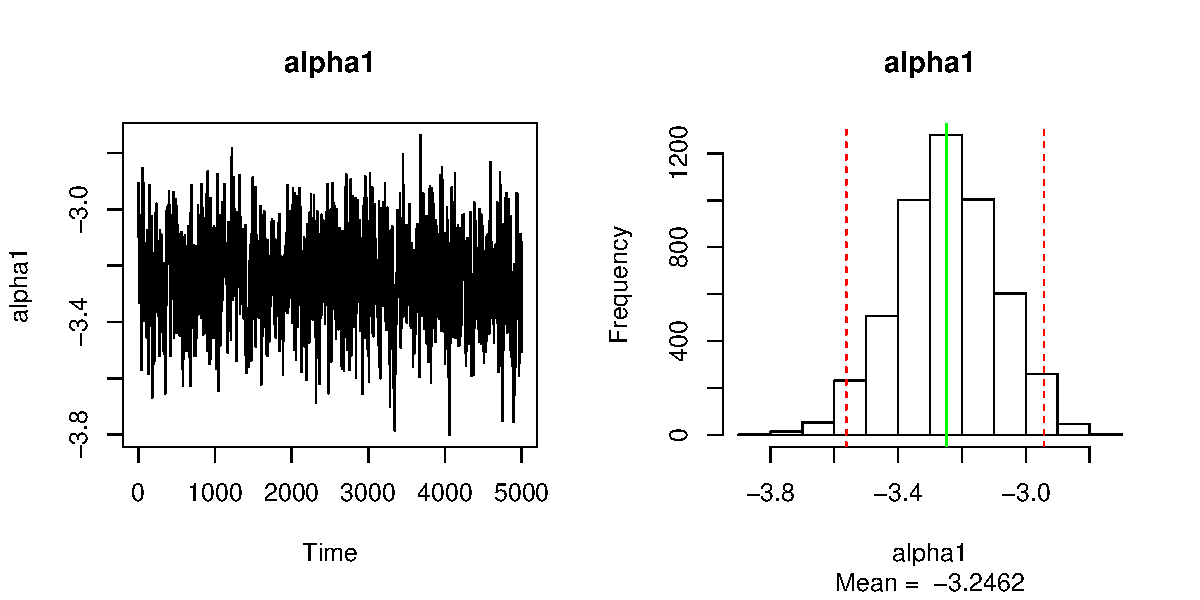
\includegraphics[scale = .7]{plot14.pdf} \\
	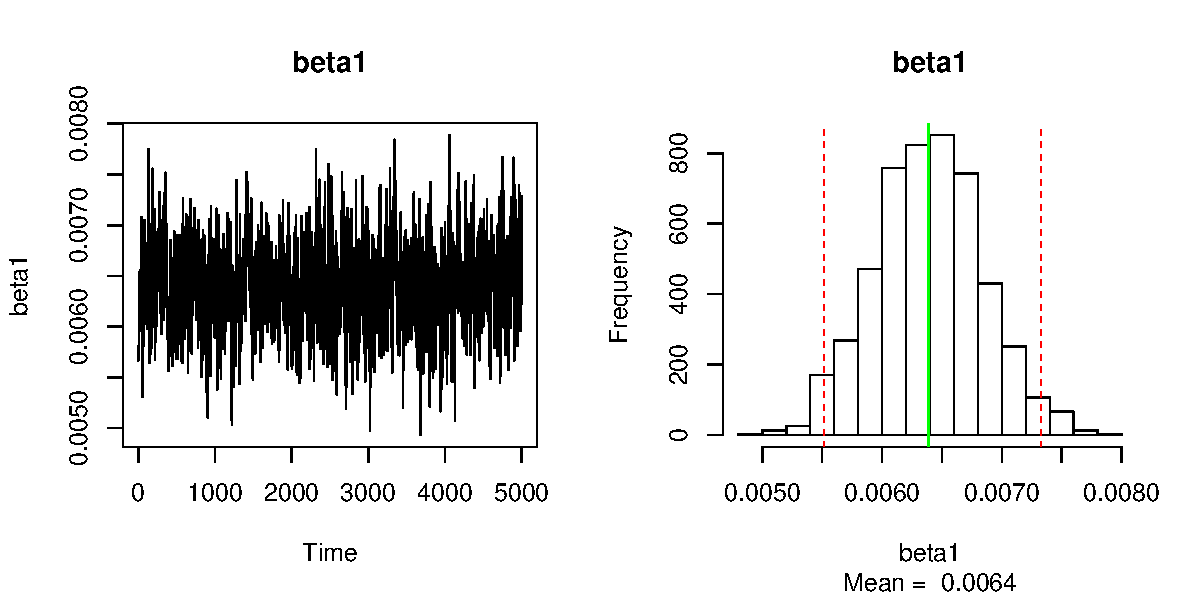
\includegraphics[scale = .7]{plot15.pdf} \\
	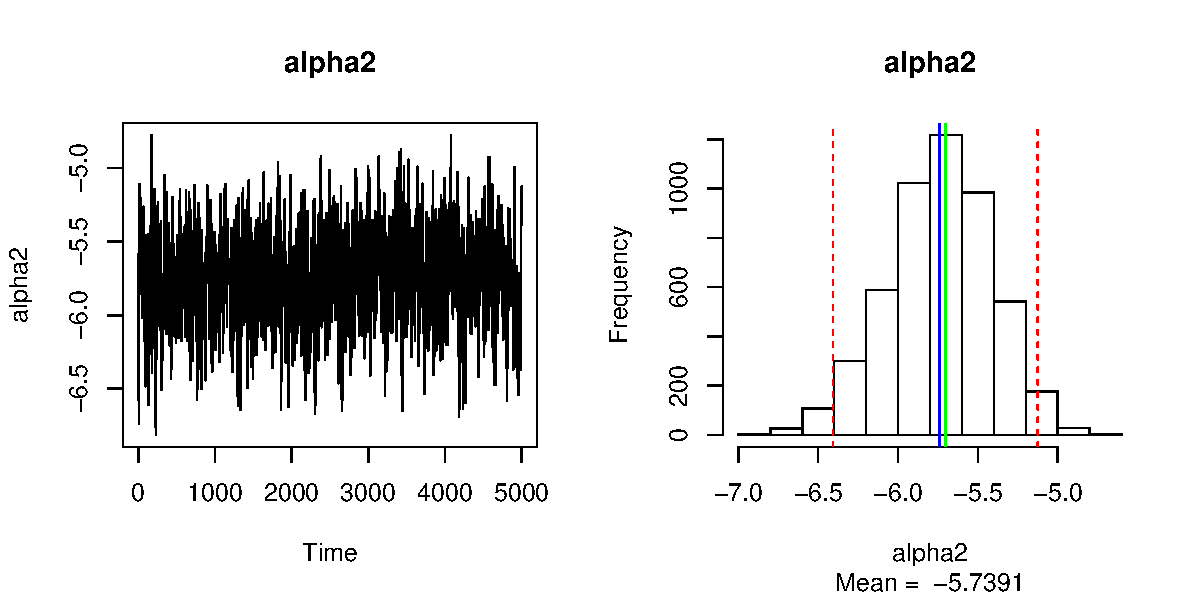
\includegraphics[scale = .7]{plot16.pdf} \\
	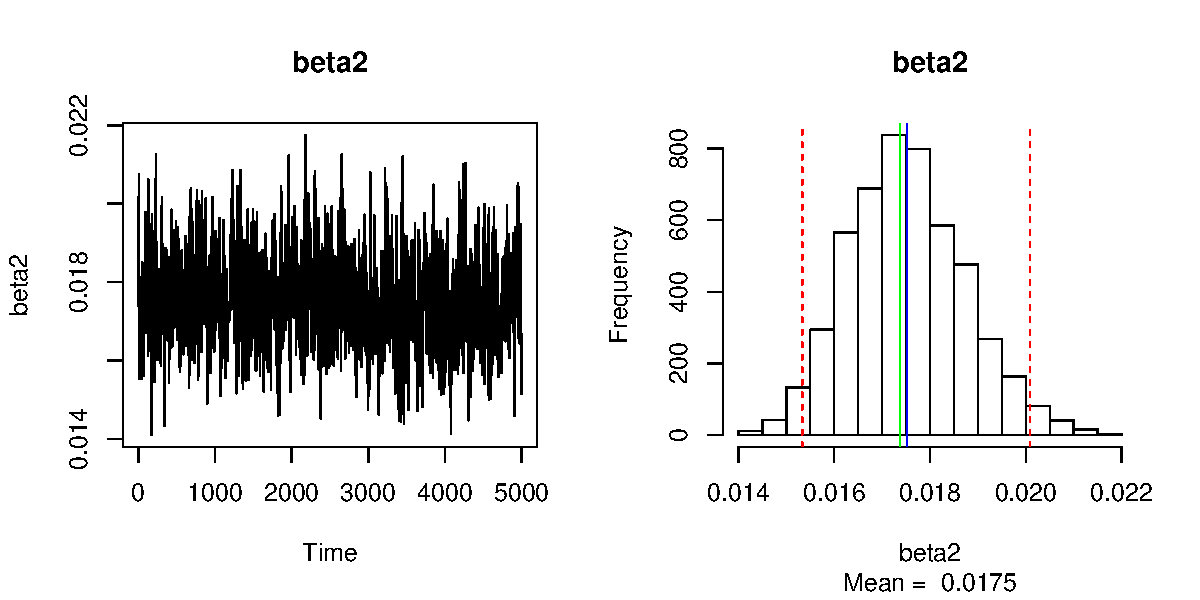
\includegraphics[scale = .7]{plot17.pdf} \\
	Using these posterior samples, we can generate point and interval estimates for the response curves $\pi_j(x)$, $j = 1,2,3$. Those response curves are plotted below. \\
	\newline
	
	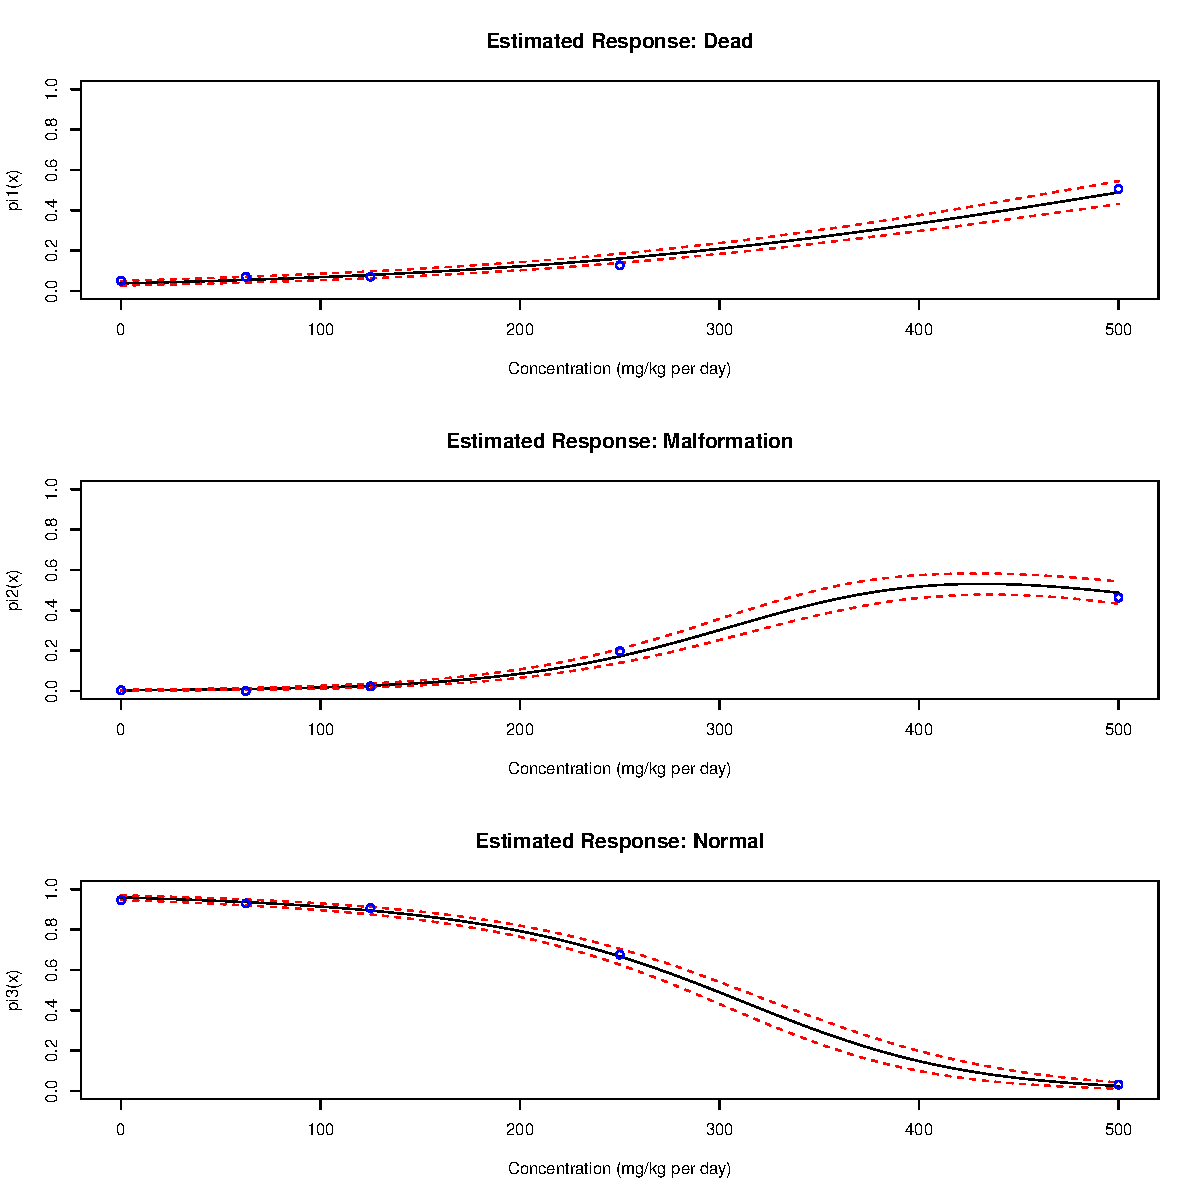
\includegraphics[scale = .7]{plot18.pdf}\\
	\newline
	We note that every observed proportion (in blue) is included in the confidence region, except for the 250 level concentration, which we noted as being farthest away from the estimated response curve earlier in this problem. 
	
	
\end{enumerate}


\end{enumerate}


\end{document}